Die Materialzufuhr besteht aus mehreren Problemstellungen. Es muss ein Probenkörper Senkrecht über dem Heizrohr befästigt werden, welcher dann vertikal verfahren werden kann.



\begin{enumerate}
    \item[]Die folgenden Bedingungen aus der Anforderungsliste sind zu erfüllen: \vspace{2mm}
    \item Die maximal zu förderende Länge eines Probenkörpers soll $500mm$ betragen (\ref{tab:anforderungsliste} Punkt 6.1)
    \item Es sollen Proformen mit Durchmessern von $10mm-45mm$ verwendbar sein (\ref{tab:anforderungsliste} Punkt 6.2).
    \item Außerdem sollen verschiedene Querschitte ( Rund, Quader) von Probenkörpern aufgenommen werden können.
\end{enumerate}

\subsection{Varianten}
Zur besseren Differenzierbarkeit werden verschiedene Varianten für die Linearführung und für die Aufnahme des Probenkörpers  diskutiert.

\subsubsection{Linearführung}
Zur Förderung von Material gibt es Prinzipiell zwei Varianten. Erstens die Probe kann mit einer Linearachse und eine entsprechenden Aktor bewegt werden. Zweitens, sie kann ,ähnlich wie bei der Faser, zwischen zwei getriebenen Rollen eingeklemmt und nach unten gefördert werden. 

\begin{enumerate}[label=(\alph*)]
    \item \textbf{Linearchse}\\
    In Abbildung \ref{fig:linearachse} ist der Aufbaue einer Linearchse dargestellt. Neben dieser Variante gäbe es noch die Möglichkeit die in der Mitte der Darstellung verwendete Trapezgewindespindel durch ein anderes System zu Ersetzen.Geeignet dafür wären sowohl Hydraulische als auch Pneumatische Zylinder. Zu beachten ist aber das der Kostenaufand für ein solchen Aktor viel größer sind. Weiterhin ist auch der Wartungsaufwand und die Fehleranfälligkeit viel größer. Das liegt zum einen daran das beide Alternativen niemals zu hundert Prozent dicht sind und es das es im Fehlerfall nicht nur zum Ausfall sondern auch zu Leckagen kommen kann, was im Falle eines Hydraulischen Systems einem großen Reperaturaufand bedeuten würde.
    \begin{figure}[!h]
        \centering
        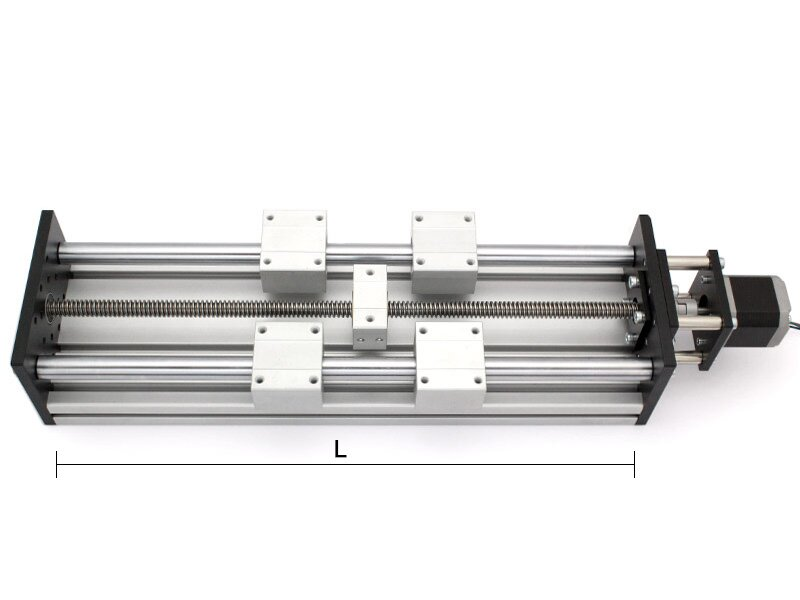
\includegraphics[width = 0.5\textwidth]{Abbildungen/linearachse-konfigurator-easy-mechatronics-system-1216a-nennlaenge-150mm~2.jpg}
        \caption{Beispiel einer Linearachse \cite{LinearachseDOLD.}}
        \label{fig:linearachse}
    \end{figure}
    
    Bei der Verwendung eines Motors in Kombination mit einer Spindel, wie in Abbildung \ref{fig:linearachse}, ist sowohl der Wartungs- als auch der Kostenaufand gering. Wenn bei diesem Aufbau der Motor ausfällt hat es keine weiteren Folgen und er kann einfach ersetzt werden. Zu diskutieren ist noch welche Art von Spindelgetriebe verwendet werden sollte. Es gibt die Variante mit Trapezgewindespindel und die mit Kugelumlaufspindel. Was den Wirkungsgrad angeht ist die Trapezgewindespindel unterlegen, da diese Gleitreibung im Gewinde besitzt. Die Kugelumlaufspindel sitzt nicht in einem klassischem Gewinde sondern wird mit wird durch eine Mutter geführt die Kugeln statt eines Gewindes besitzt. Das führt neben der geringeren Reibung auch zu einer längeren Standzeit. Nachteilig ist jedoch das sie keine Selbsthemmung besitzt und so die Achse im stromlosen Zustand nach unten fällt, da sie vertikal verbaut werden muss. Da die zuvor berechneten Kräfte und Geschwindigkeiten sehr klein sind ist der Wirkungsgrad nicht entscheidend. Der wesentliche Vorteil der Trapezgewindespindel ist der geringere preis weswegen diese für einen ersten Prototypen zu wählen ist.
    Diese Variante ist somit Preiswert und Flexibel, da auf die Achse alle möglichen arten von Materialhaltern montiert werden kann ohne die Steuerung oder das Getriebe verändern zu müssen.

    \item \textbf{Abtriebsrollen}\\
    Eine weitere möglichkeit ist ein ähnliches vorgehen wie Variante (b) bei dem Abzug. Dazu würde der Probenkörper zwischen zwei rollen geklemmt und nach unten gedrückt werden. In Abbildung \ref{fig:abtrieb_mat} ist eine Entwurf eines solchen Systems zu sehen. Es ist wichtig zu beachten das sich je nach Durchmesser des Probenkörpers die Auflagefläche in den Rollen ändert, was dazu führen kann das zu wenig Reibung vorherrscht. Deswegen wäre hier für jeden Durchmesser eine andere Aufnahme von Nöten. Dies gilt auch wenn an andere Querschnitte wie Quader gedacht wird. Vorteilhaft ist das diese Variante platzsparender ist und theoretisch beliebig lange Probenkörper zulässt.
  
    \begin{figure}[!h]
        \centering
        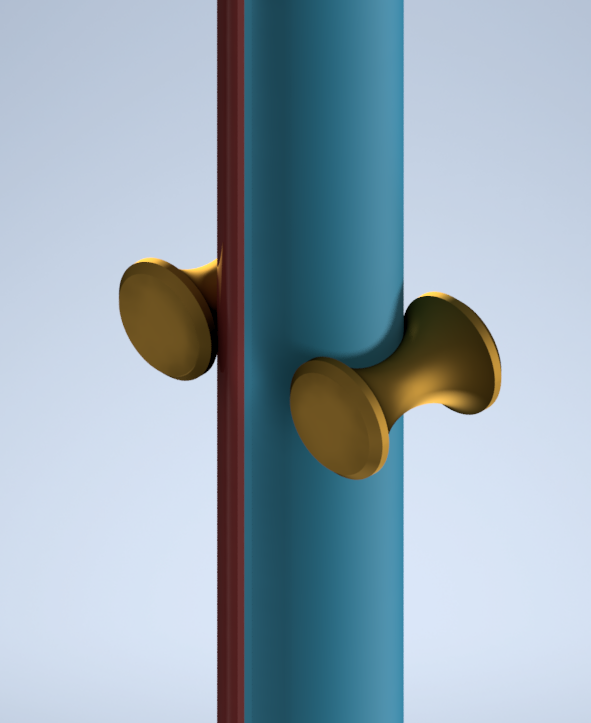
\includegraphics[width = 0.4\textwidth]{Abbildungen/abtrieb_mat.png}
        \caption{Abtriebsrollen für die Materialförderung}
        \label{fig:abtrieb_mat}
    \end{figure}
    
    \newpage
    
    \item \textbf{Auswahl}\\
    Da die Linearachse eine einfachere Modifizierbarkeit sowie besitzt und sie als fertiges Kaufteil erworben werden kann ist sie die bessere Wahl. Mit verschieden Anbauteilen lässt sich die Ache für ein breites Spektrum an Probenkörpern verwenden. 
    Das mit der Linearachse keine beliebig langen Teile verarbeitet werden können spielt bei ein Versuchstand keine Rolle da zunächst eher kleine Proben in verschieden Konfigurationen verwendet werden sollen. 



\end{enumerate}

\subsubsection{Materialhalterung}
Aus dem oberen Vergleich geht hervor das eine Linearchse verwendet wird, weshalb hier nur verschiedene Halterungen für diesen Typ Achse diskutirt werden.

\begin{enumerate}[label=(\alph*)]

\item \textbf{Spannfutter}\\
Eine möglichkeit der Befestigung ist die Verwendung eines Spannfutters, wie es auch bei einer Drehbank zum einsatz kommt. 

\begin{figure}[!h]
    \centering
    \includegraphics[width = 0.3\textwidth]{Abbildungen/Präzisions 4 Backenfutter.jpg}
    \caption{Spannfuter 160mm für Drehbänke \cite{MUK24.13.01.2024}}
    \label{fig:spannfutter}
\end{figure}

In Abblidung \ref{fig:spannfutter} ist ein solches zu sehen. Je nach Ausführung lassen sich die in der Mitte befindlich Backen auf ein variables Maß einstellen und können so verschiedenste Größen von Probenkörper aufnehmen. Werden nun noch ein paar Adapter (zum Beispiel eckig zu rund) beigelegt können auch variable Querschnitte aufgenommen werden. Ein weitere Vorteil ist das die Probe immer beim festziehen automatisch zentriert wird. Negativ zu Betrachten ist das diese futter sehr schwer sind, da sie im Originalen Einsatzfeld relativ große Kräfte aushalten müssen. Für den Versuchsstand sind sie demzufolge Überdimensioniert da die auftretenden Kräfte dort sehr klein sind.

\item \textbf{Klemmbacken}\\
Eine einfachere Variante ist der Einsatz von Klemmbacken, wie in Abbildung \ref{fig:klemm_linear}. Diese funktionieren im Prinzip wie eine Schraubzwinge. Mit einer Schraube wird eine der blauen Backen so weit in dieMitte gedreht das sich die Probe über der Mitte des Rohrofens befindet. Dann wird die zweite Seite dagegen geschoben und fixiert so die Probenkörper. Je nach dem wie viel Drehmoment auf die Vorrichtung gegeben wird können Preformen unterschiedlich stark geklemmt werden. 

\begin{figure}[!h]
    \centering
    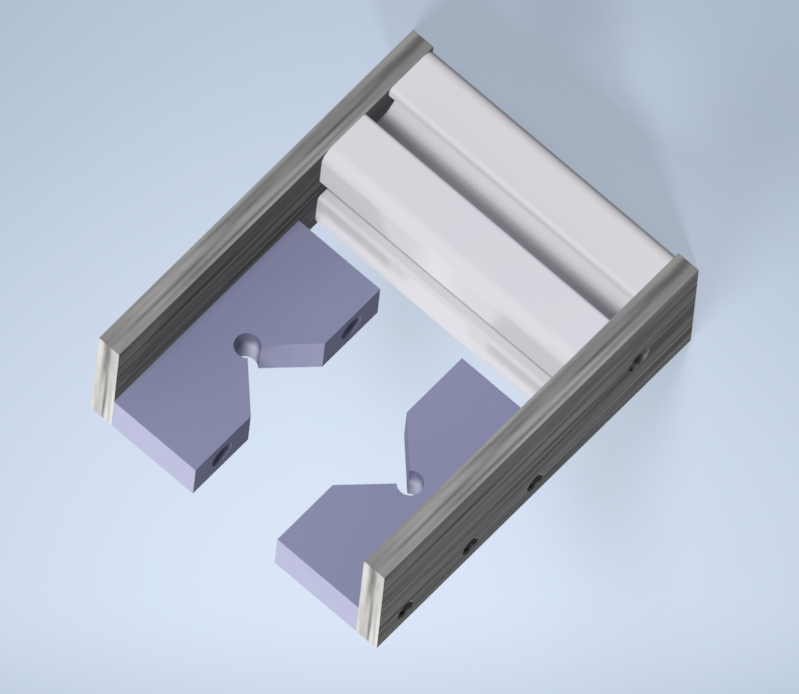
\includegraphics[width = 0.5\textwidth]{Abbildungen/aufnehmer_linear.png}
    \caption{Klemmbacken zur Halterung von Probenkörpern}
    \label{fig:klemm_linear}
\end{figure}

Diese Variante ermöglicht außerdem die Halterung von runden und eckigen Querschnitten ohne Umbau oder den Einsatz von Adaptern. Der Nachteil zu vorherigen Variante ist das der Probenkörper nicht automatisch zentriert wir, weshalb die Einrichtung einer Probe etwas schwieriger ist.

\item \textbf{Auswahl}\\
Die Erste Variante ist zwar klar die bessere, jedoch ist sie auch wesentlich teurer und schwerer. Damit der Versuchsstand so einfach und kosteneffizient wie möglich bleibt fällt die Wahl auf Variante (b), zum großen Teil auch deswegen weil sie viele verschiedene Probenkörper ermöglicht.

\end{enumerate}


\subsection{Dimensionierung und Komponentenauswahl}

\subsubsection{Linearführung}
Zur Linearführung sind alle wirkenden Lasten zu berechnen um sicherzustellen das die Trapezgewindespindel diesen Standhält. Ebenfalls muss ein Motor ausgelegt werden der die entsprechenden Lasten bewegen kann.

\begin{enumerate}[label=(\alph*)]
    \item \textbf{Axialkraft}\\
    Die einzige Last die auf das System wirkt ist jene, welche vom  Eigengewicht des Probenkörpers ausgeht.
    \begin{equation}\label{eq:mg}
        F = m\cdot g
    \end{equation}
    Die zu auf die Spindelmutter wirkende Axialkraft $F$ ergibt sich so mit Gleichung \ref{eq:mg}. Da die Masse noch Unbekannt ist muss diese Ermittelt werden. 
    \begin{equation}\label{eq:masse}
        m = \frac{\pi \cdot d^2}{4} \cdot L \cdot \rho
    \end{equation}
    Zur Abschätzung der maximalen Masse wird ein zylindrischer Probenkörper mit einem Durchmesser $d=50mm$ und einer Länge $L = 500mm$ angenommen. Die dichte der Probenkörper varriert je nach Materialkombination. Die mittlere Dichte der meisten verwendbaren Materialien liegt bei circa $1,5 \frac{g}{cm^3}$. Um auch Materialkombinationen abzudecken die nicht im Entwurf bedacht wurden wird mit einem Sicherheitsfaktor von zwei, eine maximale mittlere Dichte $\rho$ von $3,0\frac{g}{cm^3}$ angenommen.
    \begin{equation} \label{eq:F_final}
        F = \frac{\pi \cdot d^2}{4} \cdot L \cdot \rho \cdot g
    \end{equation}
    Mit Gleichung \ref{eq:F_final} und einer Fallbeschleunigung von $g =  9,81 \frac{m}{s^2}$ ergibt sich die auf die Trapezgewindemutter maximal wirkende Kraft (Gleichung \ref{eq:solve_F}).
    \begin{equation}\label{eq:solve_F}
        F = \frac{\pi \cdot (0,05m)^2}{4} \cdot 0,5m \cdot 3000\frac{kg}{m^3} \cdot 9,81\frac{m}{s^2} = 28,893N
    \end{equation}


    \item \textbf{Knickbeanspruchung}\\
    Da die Gesamte Kraft (Gleicung \ref{eq:solve_F} von der Spindel gehalten werden muss, ist sicherzustellen das diese nicht abknickt. Aus dem Datenblatt des Herstellers lässt sich so mit Gleichung \ref{eq:fcp} die maximal zulässige Kraft auf die Spindel bestimmen.
    \begin{equation}\label{eq:fcp}
        F_{cp}= \frac{21\cdot10^4\cdot D_3 \cdot \pi ^3 \cdot f}{64 \cdot L_{cp}^2} \hspace{20} \cite{DOLDMechatronikGmbH.}
    \end{equation}
    
    Im vorliegenden Fall ist jedoch der benötigte Kerndurchmesser $D_3$ die unbekannte, da die maximal wirkende Kraft zuvor bereits berechnet wurde. 
    \begin{equation}
        D_3 = \frac{F_{cp}\cdot 64 \cdot L_{cp}^2}{21\cdot 10^4 \cdot \pi^3 \cdot f}
    \end{equation}
    \begin{figure}[!h]
        \centering
        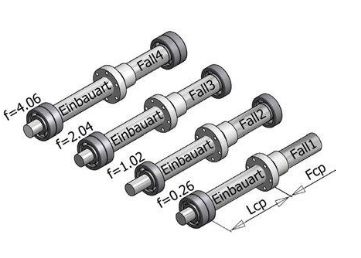
\includegraphics[width=0.5\textwidth]{Abbildungen/Lagerungstyp.png}
        \caption{Lagerungstypen für Spindeltriebe \cite{DOLDMechatronikGmbH.}}
        \label{fig:lagerung_knick}
    \end{figure}

    Angenommen wird eine Lagerung $f=1,02$ aus Abbildung \ref{fig:lagerung_knick}. Somit ergibt sich mit der Kraft aus Gleichung \ref{eq:solve_F} so wie einem maximalen Abstand zwischen Lager und Mutter von $L_{cp}~=~500mm$ der minimale Kerndurchmesser.
    \begin{equation}
        D_3 = \frac{28,893\cdot10^{-3}kN\cdot 64 \cdot (500mm)^2}{21\cdot 10^4 \cdot \pi^3 \cdot 1,02} \approx 6,93\cdot10^{-2} mm
    \end{equation}
    Da der die Kraft und dadurch der benötigte Kerndurchmesser sehr klein sind können praktisch alle Größen von Trapezgewindespindeln verwendet werden. Es wird im weiteren von einer Spindel mit einem Flankendurchmesser von $12mm$ ausgegangen.

    \item \textbf{Antriebs- und Haltemoment}\\
     Um die last bewegen zu können ist ein bestimmtes Drehmoment am Motor erforderlich. Da dieses sehr stark von der Steigung der Spindel abhängt wird die Berechnung für einen Festgelegten wert für die Steigung durchgeführt. Aus Kapitel \ref{ch:systemspeed} wissen wir das die benötigten Geschwindigkeiten sehr klein sind jedoch präzise gesteuert werden müssen. Aus diesem Grund wird die kleinste, beim gewählten Hersteller angebotene, Steigung $P$ von  $3mm$ verwendet. Da jede Art von Getriebe verlustbehaftet ist wird mit Gleichung \ref{eq:spinde_wiirkungsgrad} zunächst der Wirkungsgrad bestimmt.
     \begin{equation}\label{eq:spinde_wiirkungsgrad}
         \eta = \frac{tan(\alpha)}{tan(\alpha+\beta)} \hspace{10mm} \cite{DOLDMechatronikGmbH.}
     \end{equation}
     Um den Reibungswinkel $\beta$ und den Steigungswinkel $\alpha$ zu berechnen werden die Gleichungen \ref{eq:steig_w} und \ref{eq:reib_w} verwendet.
     \begin{align}
         &\alpha = arctan(\frac{P}{D_2\cdot \pi})  \hspace{10mm}\cite{DOLDMechatronikGmbH.}\label{eq:steig_w} \\
         &\beta = arctan(\mu G) \hspace{16mm}\cite{DOLDMechatronikGmbH.}\label{eq:reib_w}
     \end{align}
     So ergibt sich mit dem Flankendurchmesser $D_2$ von $12mm$ und einem Reibungskoeffizienten von $\mu G = 0,05$ \cite{DOLDMechatronikGmbH.} der Wirkungsgrad $\eta$ (Gleichung \ref{eq:eta}).
     \begin{equation}\label{eq:eta}
         \eta = \frac{P}{D_2\cdot \pi \cdot tan(arctan(\frac{P}{D_2  \pi})+arctan(0,005))} \approx 0,6117
     \end{equation}

     Das benötigte Antriebsmoment lässt nun für die Auslegung des Motors bestimmen.
     \begin{equation}\label{eq:FtoMa}
         M_A = \frac{F \cdot P}{2000 \cdot \pi \cdot \eta} \hspace{10} \cite{DOLDMechatronikGmbH.}
     \end{equation}

    Mit Gleichung \ref{eq:FtoMa} lässt sich das minimal nötige Drehmoment berechnen. Dazu wird für $F$ der wert aus Gleichung \ref{eq:solve_F} verwendet.
    \begin{equation}
        M_A = \frac{28,893N \cdot 3mm}{2000\pi \cdot 0,6117 } = 0,0225 Nm \approx 2,25 Ncm
    \end{equation}

    Da $\alpha$ im falle einer Geschmierten welle und einer Bronzemutter größer als $\beta$ ist, ist die Trapezgewindespindel nicht Selbsthemmend \cite{DOLDMechatronikGmbH.}. Das hat zur folge das der gewählte Motor ein neben dem berechneten Antriebsmoment auch ein ebenso großes Haltemoment vorweisen muss, damit bei perfekter Schmierung der Probenkörper im Stillstand an Ort und Stelle gehalten werden kann.
    
    \item \textbf{Komponentenauswahl}

    Da der Durchmesser der Trapezgewindespindel nicht von größere Bedeutung ist wird hier eine mit $12mm$ Flankendurchmesser und einer Steigung von $3mm$ gewählt. Anbieten würde sich für die ausgesuchte Führung ein Nema 17 bipolar-Steppermotor. Dieser hat ein Haltemoment von $51 Ncm$ und ein maximales Drehmoment von $35Ncm$ welches bei Steigerung der Drehzahl auf $1000min^{-1}$ auf circa $0,5Ncm$ sinkt (bei 24V). Damit entspricht er prinzipiell den Anforderungen. Zu Überprüfen ist nun nur noch ob die Maximaldrehzahl ausreichend ist.
    \begin{equation}
        v_1 = n_{max} \cdot P
    \end{equation}
    Damit kann der Motor eine Maximale Geschwindigkeit von $50 \frac{mm}{s}$ erreichen, was über der geforderten Geschwindigkeit von $20\frac{mm}{s}$ liegt.
    
    
    
     
    
\end{enumerate}


\subsubsection{Materialaufnahme ---Entfernen ---}
